\pdfoutput=1
\documentclass[conference]{IEEEtran}
\usepackage[utf8]{inputenc}
\usepackage[T1]{fontenc}
\usepackage{graphicx}
\usepackage{amsmath,amssymb}
\usepackage{url}
\usepackage{booktabs}
\title{Exploratory Segmentation of a Constructed Colombian Building Dataset Using K-Means}
\author{\IEEEauthorblockN{Henry David Muñoz Molina}\IEEEauthorblockA{Data Engineering and Artificial Intelligence\\Universidad Santo Tomás, Tunja, Colombia\\Data Mining -- Integrative Project Progress Report}}
\begin{document}
\maketitle
\begin{abstract}
This work develops a reproducible data-mining pipeline for an author-constructed dataset of 15,010 building records from six Colombian cities. It combines schema validation, data cleaning, exploratory analysis, an initial K-Means baseline and a reproducible official cadastral API query. The supplied file contains no detected missing values or duplicate identifiers; 267 floor-count outliers are retained provisionally and examined through sensitivity analysis. Mixed variables are represented with standardized floor counts, weighted one-hot categories and a binary compliance field. Among two to eight clusters, two maximize sampled silhouette (0.2499), producing groups of 9,893 and 5,117 records with mean floor counts of 13.00 and 32.25. Seed stability is high, but cluster separation is limited and primarily reflects height. Source-level traceability and independent validation remain unresolved. The results describe the constructed dataset and do not establish seismic safety, population representativeness or inspection priorities for actual buildings.
\end{abstract}
\begin{IEEEkeywords}
Data mining, K-Means, exploratory analysis, mixed data, building profiles, SDG 11.
\end{IEEEkeywords}
\section{Introduction}
Organizing heterogeneous building attributes can support exploratory understanding of urban infrastructure. However, producing clusters is not equivalent to measuring structural vulnerability. Meaningful interpretation requires transparent data provenance, a justified similarity representation and validation of the resulting profiles.
This project implements the Data Mining module of the integrative assignment. Its contribution is a reproducible progression from the supplied CSV to audited data, descriptive evidence and an evaluated unsupervised baseline. Only computations from the supplied file and the archived official response are reported as empirical results.

\section{Problem Statement and SDG Alignment}
\subsection{Research question and objectives}
The question is: what descriptive building profiles emerge from the constructed dataset after transparent preprocessing, and how robust are they to initialization and selected preprocessing decisions?
The general objective is to characterize and segment the available records. Specific objectives are to (1) validate schema and quality, (2) examine marginal distributions and associations, (3) evaluate alternative cluster counts and (4) interpret results without equating clusters to engineering diagnoses.
\subsection{SDG 11}
The work is conceptually aligned with SDG 11, particularly resilient settlements and disaster-related loss reduction under target 11.5 \cite{un}. Organizing information could support later expert review. No SDG indicator, reduction in disaster losses or demonstrated policy impact is estimated here. A future operational system would require verified observations, engineering criteria and institutional validation.

\section{Dataset and Provenance}
\subsection{Scope and origin}
The author describes the dataset as his own construction combining several sources, including information from DANE; the integrated dataset is not publicly published. Exact source titles, URLs, extraction dates, licenses and integration rules were not supplied for this analysis. Consequently, DANE is not cited as the provider of the complete dataset. It remains unverified whether each row represents an observed building, a constructed combination or a simulated case. This limits external validity and must be resolved before making empirical claims about Colombian buildings.
The input is \texttt{08\_dataset\_simplificado.csv}, containing 15,010 rows and nine columns. The unit encoded by each row is a building record identified by a unique ID. The input hash is recorded in \texttt{results/summary.json}; the original file is preserved.
\begin{table}[ht]
\caption{Data dictionary and analytical role}
\centering\footnotesize
\begin{tabular}{p{.28\columnwidth}p{.28\columnwidth}p{.26\columnwidth}}\toprule
Field & Representation & Role \\\midrule
Building ID & Unique text & Audit only\\
City & Six categories & Profile only\\
Building use & Six categories & Clustering\\
Floors & Integer, 5--55 & Clustering\\
Structural system & Four categories & Clustering\\
Seismic threat & Three categories & Clustering\\
Recorded compliance & Yes/no & Clustering\\
Age & Four age bands & Clustering\\
Metal-structure potential & Four levels & Profile only\\\bottomrule
\end{tabular}
\end{table}
Age bands are 0--10, 11--25, 26--40 and over 40 years. Exact ages, construction years, percentages of reinforced concrete and quantitative compliance indices are not available. They are not fabricated from the categorical fields.

\subsection{Official sources and traceable external data}
Three official sources were reviewed as candidates, not as verified origins of the supplied rows. DANE's CEED provides construction-related fields and a data dictionary \cite{ceed}; it is the closest candidate for comparing building attributes. The SGC national seismic-hazard map provides territorial context \cite{sgc}. Bogota's cadastral construction layer offers floor count, height and geometry for a city-specific comparison \cite{catastro}. The cadastral service was queried for grouped floor-count statistics and used for an independent descriptive contrast. No building-level join was performed, and the baseline clusters still use only the constructed dataset. Source identifiers, periods and compatible observation units must be established before integration. Neither geographic threat nor a licensing field certifies a building's seismic compliance.

\section{Methodology and System Structure}
\subsection{Reproducible pipeline}
The system is a local analytical pipeline: immutable input CSV; schema and domain validation; cleaned CSV; exploratory tables and figures; numerical representation; K-Means selection and sensitivity checks; labeled CSV and report. The standalone Python script and executed notebook implement the same nine stages. Random seeds, dependency versions, input hash and execution output are included. No cloud infrastructure is required by the selected module. The optional external-source component is implemented as a read-only REST API query, with raw response, parameters, retrieval time and SHA-256 archived. Offline replay is the default; explicit refresh obtains a new response.
\begin{figure}[ht]\centering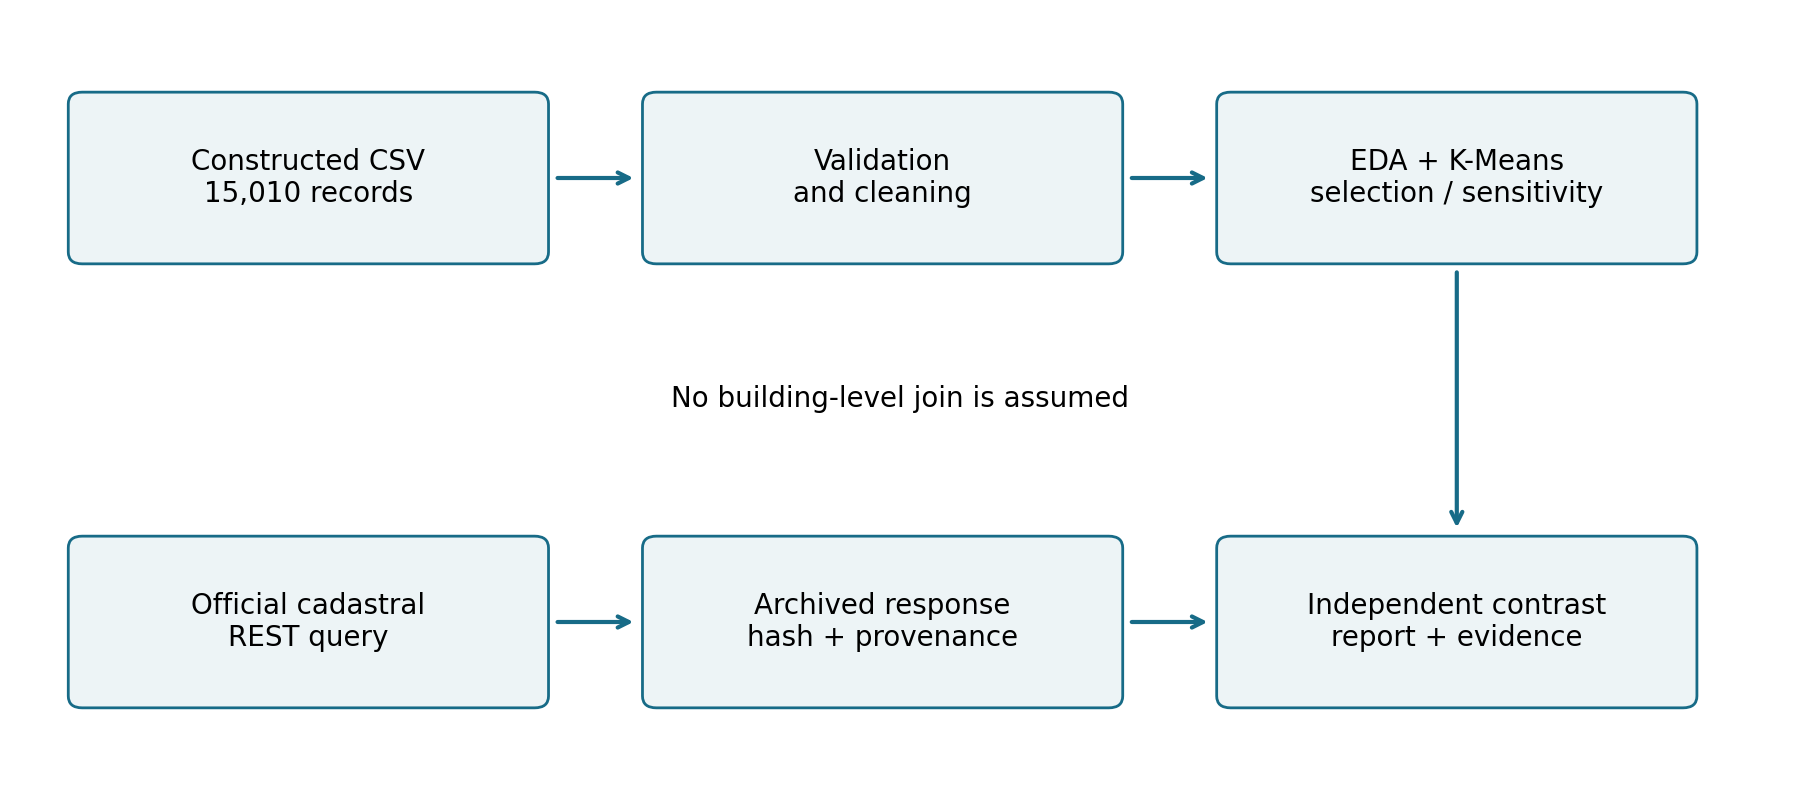
\includegraphics[width=\columnwidth]{../figures/09_system.png}\caption{Analytical system with a separate, traceable official-data branch.}\end{figure}
\subsection{Quality management}
Text is stripped of outer whitespace and empty strings are treated as missing. The pipeline checks expected columns, allowed categories, positive integer floor counts, identifier format and uniqueness. Unexpected data cause an explicit error instead of silent imputation or reassignment. No missing values or duplicates were found; therefore no imputation or deletion was necessary. Metal-potential labels are standardized and compliance is mapped to Boolean values.
For floors, $Q_1=10$, $Q_3=26$ and $IQR=16$. Tukey fences are $[-14,50]$, flagging 267 records (1.78\%) with 51--55 floors. These records are retained provisionally because a statistical outlier is not necessarily an error; their real-world validity has not been confirmed. All flagged rows are exported for source review. A sensitivity run clips floors to the fences without changing the baseline dataset.
The CSV preserves values, but not pandas categorical metadata. The script explicitly recreates model encodings on every run rather than assuming that CSV export preserves ordered types.
\subsection{Exploratory analysis}
The analysis includes numerical summaries, histogram and boxplot; categorical frequencies; city-level counts and compliance rates; compliance cross-tabulations by city, age, structural system and seismic threat; and bias-corrected Cramér's V for categorical associations. These are descriptive statistics of the available file. No population confidence interval is reported because the sampling design is unknown.
\subsection{Feature representation}
K-Means minimizes within-cluster squared Euclidean distances \cite{kmeans}. Its application to mixed data is a modeling choice, not an assumption that all categories possess physical distances. Building use, structural system, age band and threat are one-hot encoded \cite{onehot}. Every one-hot block is divided by $\sqrt{2}$, so a mismatch in one categorical variable contributes one unit to squared distance. Floor counts are standardized using their mean and population standard deviation. Compliance is encoded as zero or one and is not standardized, avoiding inflation of a rare positive category.
Thus the representation has 19 dimensions: one standardized numerical feature, 17 one-hot columns and one binary feature. The squared distance is
\begin{equation}
 d^2(i,j)=(z_i-z_j)^2+\sum_{v=1}^{4}\mathbb{I}(x_{iv}\ne x_{jv})+(b_i-b_j)^2.
\end{equation}
The ID is excluded because it is an identifier. City is excluded to avoid duplicating the nearly deterministic city--threat association. Metal-structure potential is excluded because its construction rule is unknown and may encode other features. It is used only to describe groups. Age bands are not converted to invented exact years. A sensitivity run halves the squared-distance weight of floors.
\subsection{Cluster selection and evaluation}
Candidates $k=2,\ldots,8$ use K-Means++, 20 initializations, seed 42 and a maximum of 300 iterations. All 15,010 records are used for fitting. Silhouette is computed on the same random sample of 2,500 records for every candidate; this limits computational cost and makes comparisons consistent. Maximum sampled silhouette determines the selected $k$. Inertia, Davies--Bouldin and Calinski--Harabasz indices are complementary diagnostics, not classification accuracy.
Stability is assessed with seeds 7, 21 and 84 using the adjusted Rand index (ARI) against the baseline partition. Three feature/preprocessing sensitivity tests use the selected $k$: IQR clipping, half floor weight and removal of the unverified compliance field. These checks are not independent external validation or proof of generalization. PCA is fitted only to visualize the representation, not to train the clusters.

\section{Results}
\subsection{Descriptive findings}
Floor count has mean 19.56, median 18, sample standard deviation 11.13 and range 5--55. Apartments account for 8,247 records (54.94\%); reinforced concrete is recorded in 7,265 (48.40\%). The recorded compliance field is positive in 928 rows (6.18\%) and negative in 14,082 (93.82\%). This is not a measured national noncompliance rate.
\begin{figure}[ht]\centering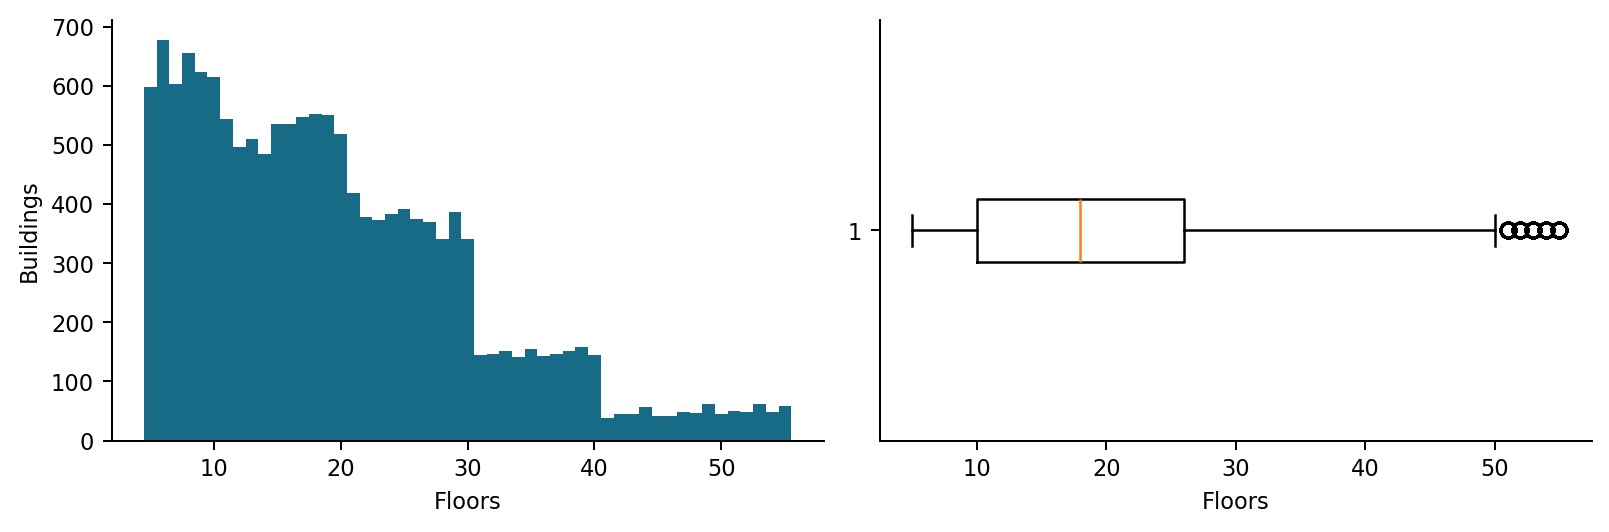
\includegraphics[width=\columnwidth]{../figures/01_floors.png}\caption{Floor-count distribution and outliers in the supplied file.}\end{figure}
\begin{table}[ht]\centering\caption{City composition and recorded compliance}\footnotesize
\begin{tabular}{lrr}\toprule City & Records & Compliance (\%)\\\midrule
Bogotá & 4,003 & 0.075\\
Medellín & 2,703 & 0.000\\
Cali & 2,503 & 0.000\\
Barranquilla & 2,101 & 24.607\\
Bucaramanga & 1,900 & 0.000\\
Cartagena & 1,800 & 22.667\\\bottomrule\end{tabular}\end{table}
City and threat have bias-corrected Cramér's V approximately 0.9999, indicating near-total association within the file. City--compliance and threat--compliance associations are approximately 0.4314 and 0.4312. The concentration of recorded compliance in Barranquilla and Cartagena, together with zero positive values in three cities, warrants review of source integration and field-construction rules. These patterns do not establish causal relationships or city-level structural safety.
\begin{figure}[ht]\centering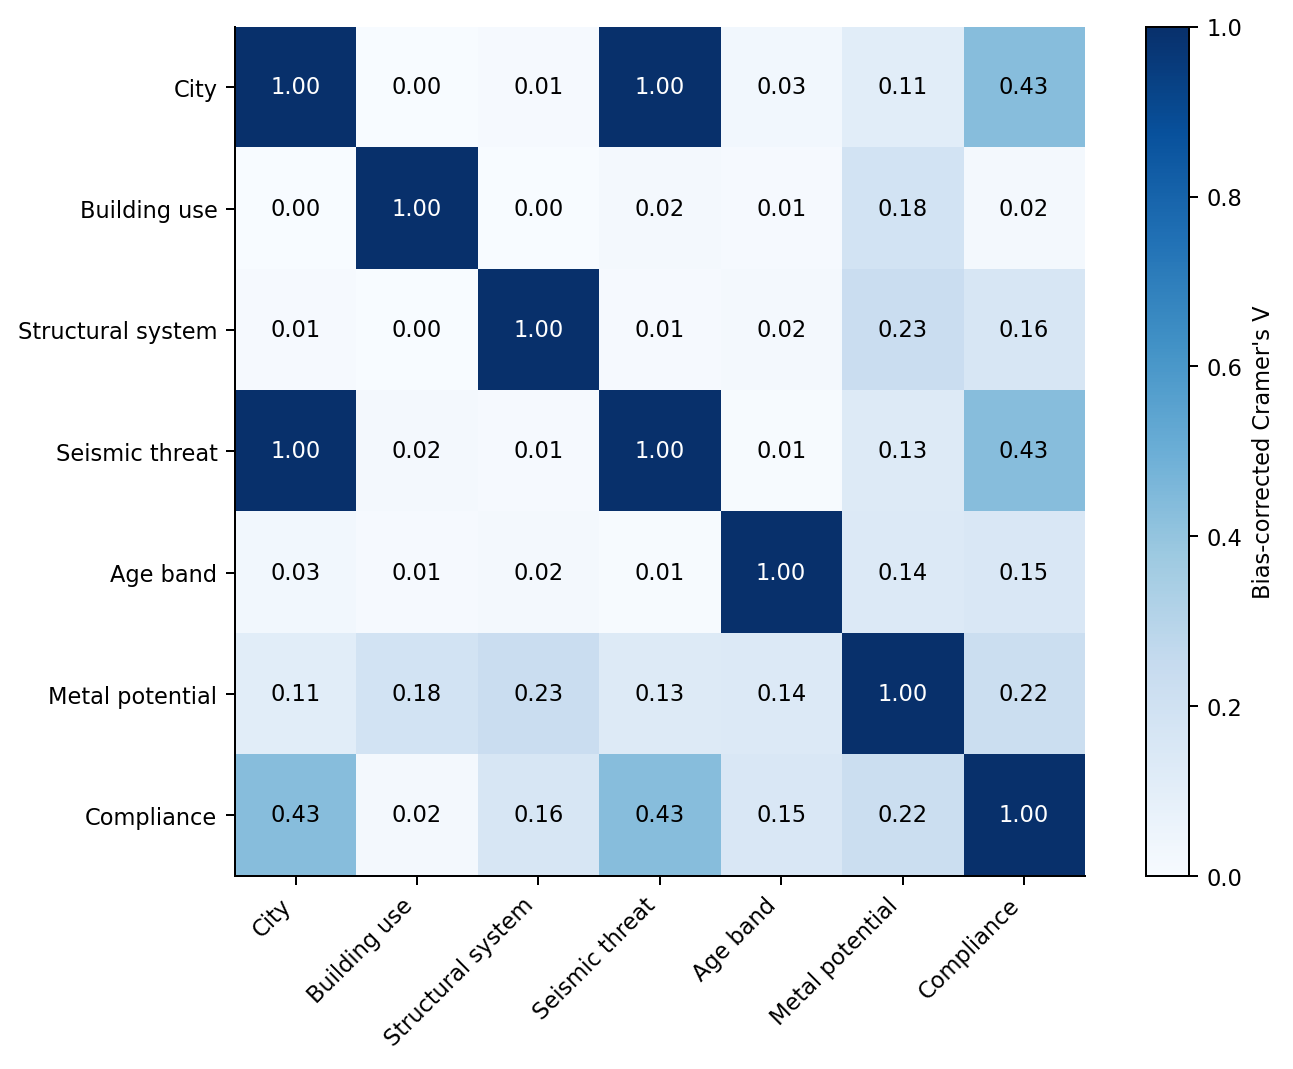
\includegraphics[width=\columnwidth]{../figures/04_associations.png}\caption{Categorical associations. Near-deterministic relationships may reflect construction rules rather than independent evidence.}\end{figure}
\subsection{Selected clustering solution}
Two clusters maximize sampled silhouette at 0.2499. The score indicates limited separation; no strongly separated risk classes are claimed. The two-cluster solution also has the lowest Davies--Bouldin and highest Calinski--Harabasz values among the tested candidates. The illustrative five-cluster result is not reproduced by forcing its group count.
\begin{table}[ht]\centering\caption{Internal evaluation on the specified representation}\footnotesize
\begin{tabular}{rrrrr}\toprule $k$ & Inertia & Silhouette & DB & CH\\\midrule
2 & 25814.6 & .2499 & 1.509 & 5917.1\\
3 & 23142.2 & .1567 & 1.937 & 4166.5\\
4 & 21688.9 & .1212 & 2.202 & 3298.7\\
5 & 20664.2 & .1165 & 2.382 & 2782.6\\
6 & 19478.5 & .1369 & 2.196 & 2544.1\\
7 & 18937.7 & .1270 & 2.215 & 2251.9\\
8 & 18171.7 & .1352 & 2.078 & 2101.7\\\bottomrule\end{tabular}
\end{table}
\begin{figure}[ht]\centering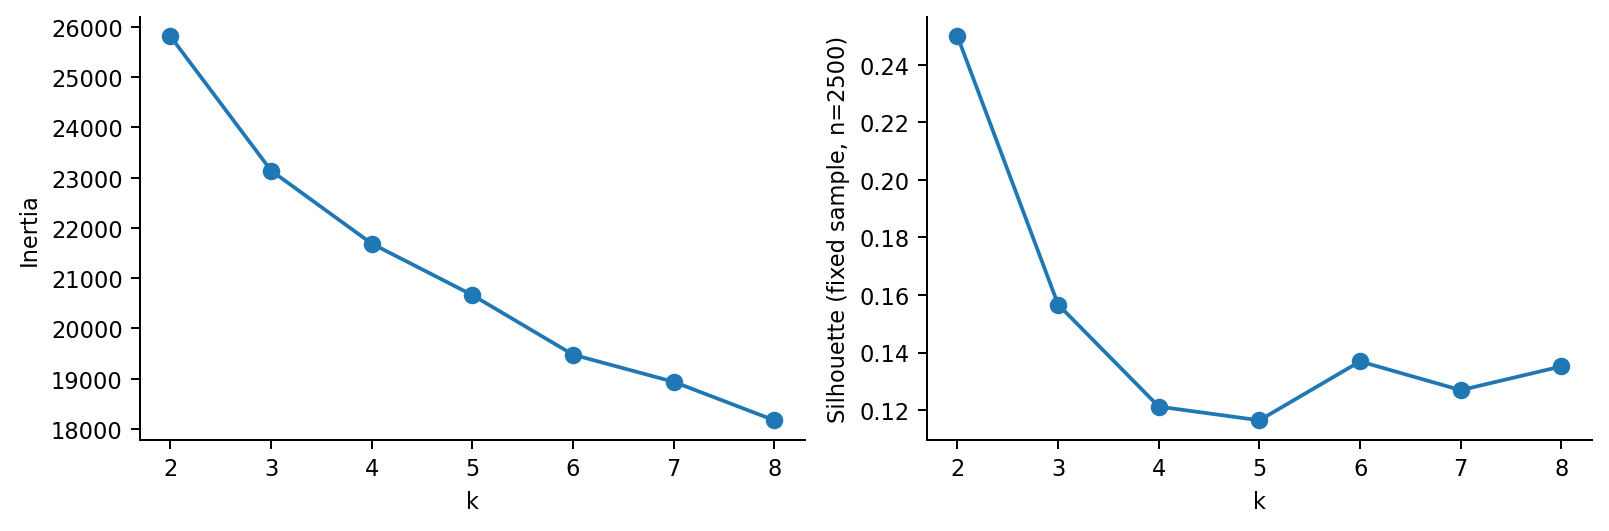
\includegraphics[width=\columnwidth]{../figures/05_selection.png}\caption{Inertia and sampled silhouette across candidate cluster counts.}\end{figure}
\begin{table}[ht]\centering\caption{Descriptive cluster profiles}\footnotesize
\begin{tabular}{lrr}\toprule & Cluster 0 & Cluster 1\\\midrule
Records & 9,893 & 5,117\\
Share (\%) & 65.91 & 34.09\\
Mean floors & 13.00 & 32.25\\
Median floors & 13 & 29\\
Recorded compliance (\%) & 6.51 & 5.55\\
Modal metal potential & Media & Alta\\\bottomrule\end{tabular}
\end{table}
Both groups share apartments, reinforced concrete, the 26--40-year age band and intermediate threat as their modal categories. The principal separation is therefore height. Neutral labels, ``lower floor-count profile'' and ``higher floor-count profile'', are appropriate; labels such as safe, deficient or rehabilitated are unsupported.
\subsection{Robustness}
ARI is 1.000 for each tested alternative seed. IQR clipping also gives ARI 1.000, so the baseline assignment is unchanged in that experiment. Halving the squared-distance weight of floors yields ARI 0.9221, showing strong but incomplete agreement and confirming some dependence on representation. Removing the compliance field at fixed $k=2$ yields ARI 1.0000 relative to the baseline and sampled silhouette 0.2545. These results support computational repeatability within this dataset rather than structural validity.

\subsection{Executed external-source module}
A read-only ArcGIS REST query grouped the official Bogota construction layer by floor count and counted its object identifiers. No names, addresses or building-level geometry were downloaded. The archived response contains 52 groups representing 2,422,631 cadastral features; 16,339 features have missing or non-positive floor counts and are excluded only from the positive-floor descriptive comparison. The remaining 2,406,292 features have weighted mean 2.11 floors. By comparison, the constructed file has 4,003 Bogota records with mean 19.58 floors and none below five floors.
The contrast is descriptive: a cadastral feature need not correspond to an independent building, and coverage, extraction dates and selection criteria differ. Consequently, the discrepancy does not establish incorrect values in individual rows or estimate citywide structural risk. It demonstrates that representativeness cannot be assumed. The response was retrieved on November 14, 2026; the exact UTC timestamp, endpoint, parameters and hash are included in the provenance manifest. Replay and a refreshed query are separate operations because the live service may change.
\begin{figure}[ht]\centering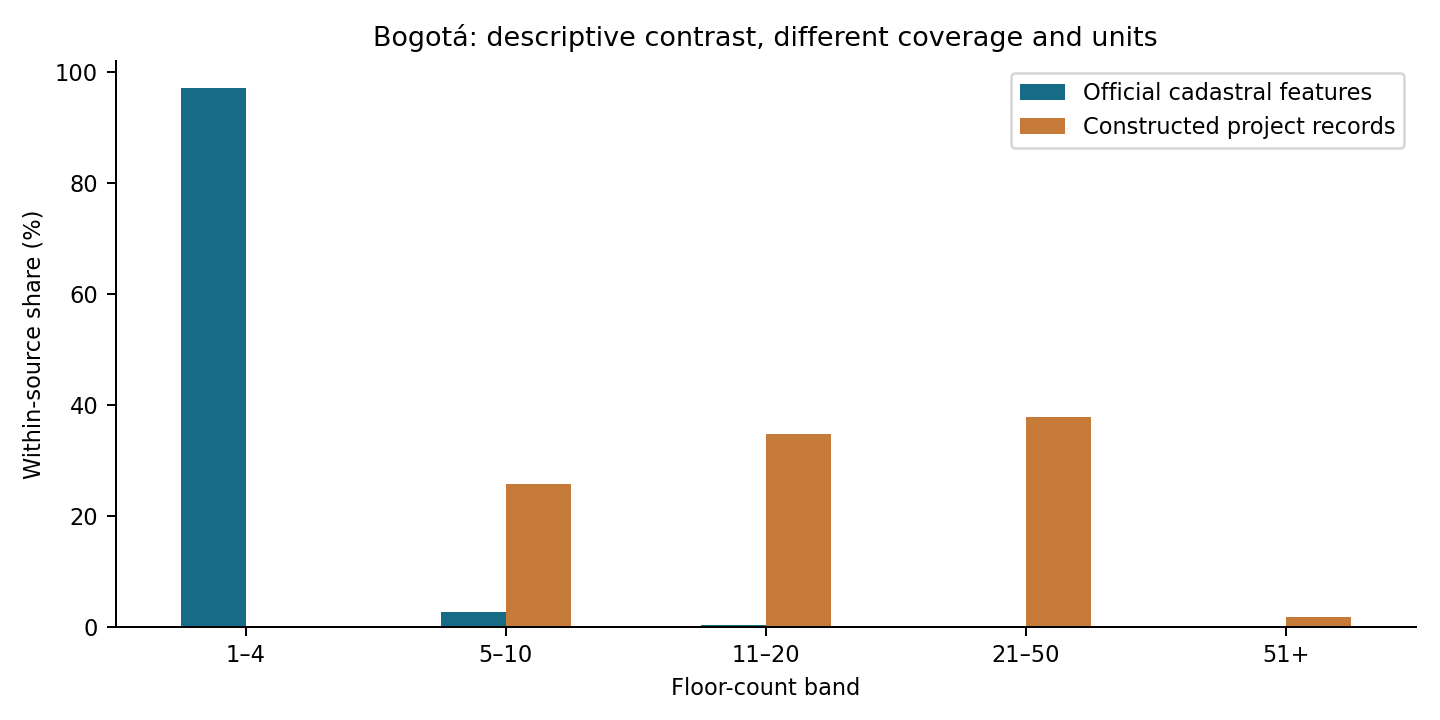
\includegraphics[width=\columnwidth]{../figures/08_external_comparison.png}\caption{Within-source floor-band shares. Different units and coverage prevent interpreting this as a matched validation sample.}\end{figure}

\section{Discussion and Limitations}
The pipeline meets the analytical scope of an initial unsupervised-mining advance: it produces auditable preprocessing, broad EDA, fitted clustering, comparative metrics and interpretable outputs. Nevertheless, substantive limitations remain.
First, provenance is incomplete. The author must identify each source and document the variables extracted, their original aggregation level, join keys and any synthetic or inferred assignments. Second, compliance and metal potential lack verified construction definitions; compliance cannot be treated as certified structural performance. Third, one-hot Euclidean geometry ignores order and engineering meaning in threat and age categories. The chosen metric is transparent but not uniquely correct. Fourth, a single numerical variable strongly influences the groups; future work can compare mixed-data dissimilarities or categorical/mixed clustering algorithms. Fifth, sampled silhouette, seed checks and the sensitivity tests do not replace resampling validation, domain expertise or independent data.
The source-data table and repository submission remain administrative and evidentiary tasks for the author. The official API-consumption module is complete; publication to the course repository and campus submission are outside the executed local pipeline.

\section{Conclusions and Next Steps}
All 15,010 records were retained after validation, with 267 high-floor observations explicitly flagged for source review. The selected two-cluster baseline is stable to tested seeds and clipping, but its limited silhouette and predominantly height-based separation constrain interpretation. The analysis demonstrates reproducible data-mining practice without making unsupported claims about seismic safety.
The immediate priorities are to complete source traceability, verify field-construction rules, review anomalous compliance patterns and publish the reproducible materials to the course repository. Expert validation and alternative mixed-data methods are subsequent methodological improvements. This report addresses the supplied progress guidelines; it does not assume additional final-project requirements that have not been provided.
\begin{thebibliography}{9}
\bibitem{un} United Nations, ``Goal 11: Sustainable cities and communities,'' Department of Economic and Social Affairs. Accessed: Nov. 14, 2026. [Online]. Available: \url{https://sdgs.un.org/goals/goal11}
\bibitem{kmeans} Scikit-learn developers, ``KMeans,'' API documentation. Accessed: Nov. 14, 2026. [Online]. Available: \url{https://scikit-learn.org/stable/modules/generated/sklearn.cluster.KMeans.html}
\bibitem{onehot} Scikit-learn developers, ``OneHotEncoder,'' API documentation. Accessed: Nov. 14, 2026. [Online]. Available: \url{https://scikit-learn.org/stable/modules/generated/sklearn.preprocessing.OneHotEncoder.html}
\bibitem{course} Universidad Santo Tomás, Tunja, ``Lineamientos de entrega de avance -- Proyecto integrador: Modalidad modular y flexible,'' course handout, 2026. Supplied by the author.
\bibitem{ceed} DANE, ``Censo de Edificaciones -- CEED,'' catalog and data dictionary. Accessed: Nov. 14, 2026. [Online]. Available: \url{https://microdatos.dane.gov.co/index.php/catalog/873}
\bibitem{sgc} Servicio Geologico Colombiano, ``Mapa de Amenaza Sismica Nacional,'' geoservice. Accessed: Nov. 14, 2026. [Online]. Available: \url{https://srvags.sgc.gov.co/arcgis/rest/services/Amenaza_Sismica/Amenaza_Sismica_Nacional/MapServer}
\bibitem{catastro} Unidad Administrativa Especial de Catastro Distrital, ``Construccion,'' Bogota geographic layer. Accessed: Nov. 14, 2026. [Online]. Available: \url{https://sig.catastrobogota.gov.co/arcgis/rest/services/catastro/construccion/MapServer/0}
\end{thebibliography}
\end{document}
